\chapterimage{chapter_head_2.pdf} % Chapter heading image

\chapter{Preliminaries}

\section{Ciphers}
%\index{Paragraphs of Text}
\subsection{Stream Cipher}
For stream ciphers Tor uses 128-bit AES in counter mode, with an IV of all 0 bytes.
\\
Here we provide some notes about AES counter mode:

\subsubsection{AES}

AES is based on a design principle known as a substitution–permutation network, and is efficient in both software and hardware.
\\
\\
\textbf{High-level description of the algorithm}:
\begin{enumerate}
	\item KeyExpantion: round keys are derived from the cipher key using Rijndael's key schedule. AES requires a separate 128-bit round key block for each round plus one more.
	\item Initial round key addition:
		\begin{enumerate}
			\item AddRoundKey: each byte of the state is combined with a block of the round key using bitwise xor.
		\end{enumerate}
	\item For 9, 11 or 13 rounds:
		\begin{enumerate}
			\item SubBytes: a non-linear substitution step where each byte is replaced with another according to a lookup table.
			\item ShiftRows: a transposition step where the last three rows of the state are shifted cyclically a certain number of steps.
			\item MixColumns: a linear mixing operation which operates on the columns of the state, combining the four bytes in each column.
			\item AddRoundKey
		\end{enumerate}
	\item Final round (making 10, 12 or 14 rounds in total):
		\begin{enumerate}
			\item SubBytes
			\item ShiftRows
			\item AddRoundKey
		\end{enumerate}
\end{enumerate}
\pagebreak
In cryptography, a block cipher by itself is only suitable for the secure cryptographic transformation (encryption or decryption) of one fixed-length group of bits called a block. A mode of operation describes how to repeatedly apply a cipher's single-block operation to securely transform amounts of data larger than a block.
\subsubsection{Counter mode encryption}
The figure \ref{fig:AES_CTR} will show a block cipher encryption with counter mode operation.


\begin{figure}[!h]
\centering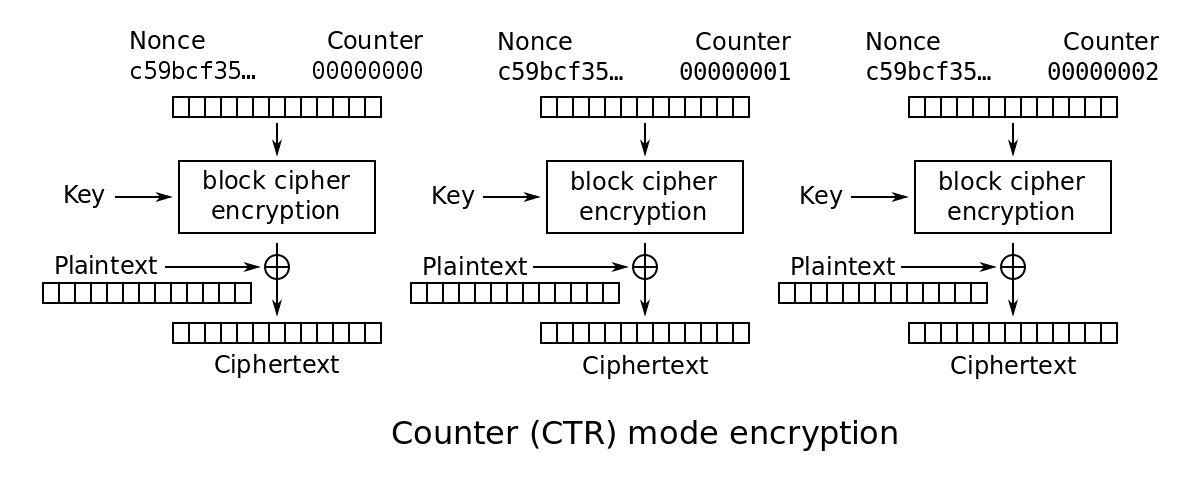
\includegraphics[scale=0.35]{AES_cntr}
\caption{AES counter mode}
\label{fig:AES_CTR} % Unique label used for referencing the figure in-text
\end{figure}

Note that the nonce in this diagram is equivalent to the initialization vector (IV) in the other diagrams. However, if the offset/location information is corrupt, it will be impossible to partially recover such data due to the dependence on byte offset.
\\
\linebreak
You can see details of counter mode in figure \ref{fig:AES_cntr_kh}.

\begin{figure}[!h]
\centering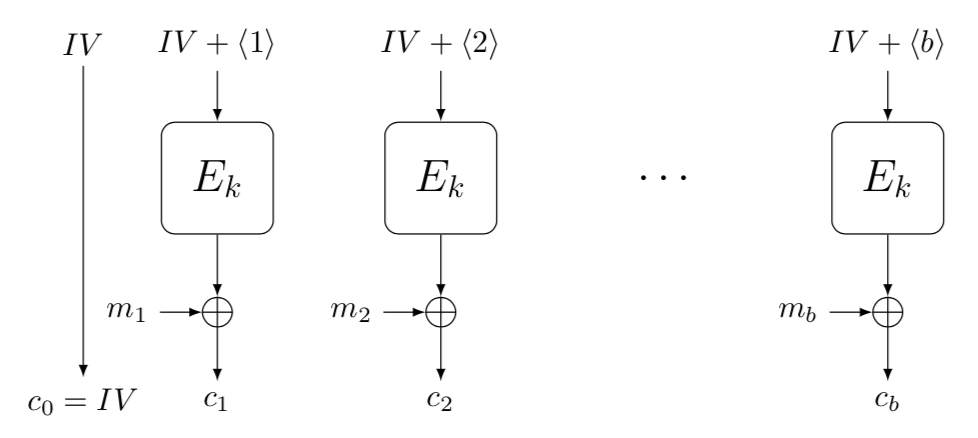
\includegraphics[scale=0.8]{AES_cntr_kh}
\caption{AES counter mode}
\label{fig:AES_cntr_kh} % Unique label used for referencing the figure in-text
\end{figure}

At first, should choose an IV randomly from $\{0,1\}^n$ then the purpose is finding every c in this way:
\\
\begin{center}
$c_i = m_i\ \oplus\ E(IV + <i>),\ i = 1,2,...,b$	
\end{center}
In the above equation $<i>$ will illustrate binary format for number $i$, also $IV+<i>$ is modular summation with the base of $2^n$.
\linebreak
One of the advantages for CTR operation mode is that we can pararellize the encryption and decryption procedure in this mode.
%\lipsum[1-7] % Dummy text

%------------------------------------------------

\section{Citation}\index{Citation}

This statement requires citation \cite{article_key}; this one is more specific \cite[162]{book_key}.

%------------------------------------------------

\section{Lists}\index{Lists}

Lists are useful to present information in a concise and/or ordered way\footnote{Footnote example...}.

\subsection{Numbered List}\index{Lists!Numbered List}

\begin{enumerate}
\item The first item
\item The second item
\item The third item
\end{enumerate}

\subsection{Bullet Points}\index{Lists!Bullet Points}

\begin{itemize}
\item The first item
\item The second item
\item The third item
\end{itemize}

\subsection{Descriptions and Definitions}\index{Lists!Descriptions and Definitions}

\begin{description}
\item[Name] Description
\item[Word] Definition
\item[Comment] Elaboration
\end{description}
